\begin{frame}[t]{1944 draft margins: internal and external response}
\tiny\centering
\begin{threeparttable}
\begin{tabular}{lccccc}
\toprule
 & Total internal & Retention & Same dept. & Diff. dept. & External hires \\
\midrule
Male drafted workers & 0.193$^{***}$ & 0.071$^{**}$ & 0.059$^{**}$ & 0.063$^{***}$ & 0.097$^{***}$ \\
 & (0.056) & (0.036) & (0.026) & (0.012) & (0.034) \\
\midrule
Observations & \multicolumn{5}{c}{623} \\
Offices clustered & \multicolumn{5}{c}{161} \\
Section and occupation FE & \multicolumn{5}{c}{Yes} \\
Log cumulative male baseline & \multicolumn{5}{c}{Yes} \\
\bottomrule
\end{tabular}
\begin{tablenotes}[flushleft]
\tiny\item \textit{Notes:} OLS, 1944 only. Unit: observed destination office $\times$ team $\times$ occupation cell, with section identifiers retained. Outcomes exclude male workers marked drafted in 1944. Exposure is the male draft count in the same office-team-occupation cell. Cells without observed non-draftee outcomes are outside the sample. These are conditional associations, not identified causal replacement effects. Internal total includes retention, same-department transfers, and different-department transfers. Standard errors clustered by office. $^{***}p<0.01$, $^{**}p<0.05$, $^{*}p<0.1$.
\end{tablenotes}
\end{threeparttable}
\vspace{2mm}
\par Internal / external $= 0.1932 / 0.0967 = \mathbf{2.00:1}$.
\end{frame}

\begin{frame}[t]{1944 draft margins: decomposition}
\centering
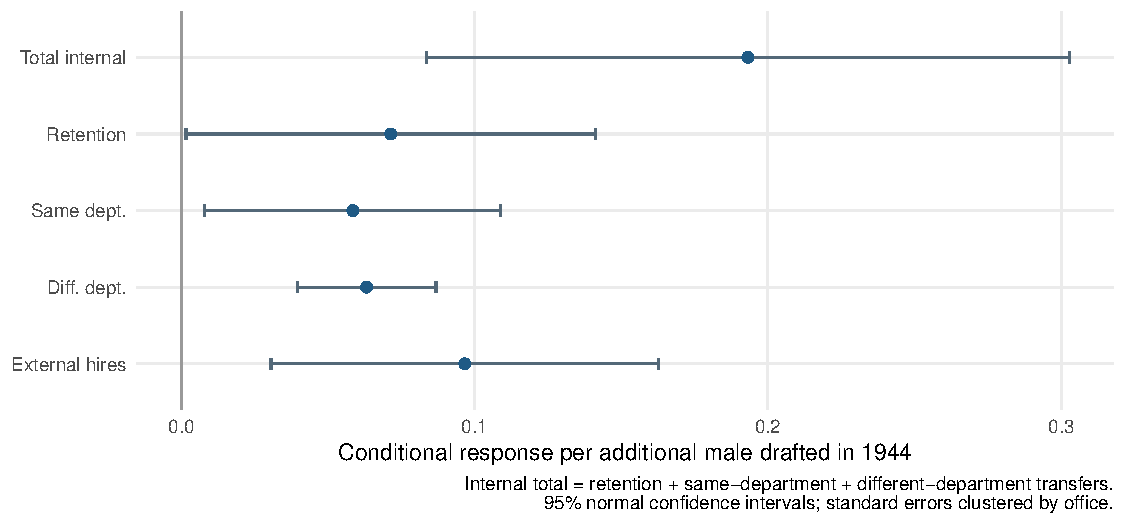
\includegraphics[width=0.92\textwidth]{Results/draft1944_pre_draft_trajectories/replacement_margins_1944.pdf}
\end{frame}

\begin{frame}[t]{Draft margins: pooled 1938--1945 benchmark}
\tiny\centering
\begin{threeparttable}
\begin{tabular}{lccccc}
\toprule
 & Total internal & Retention & Same dept. & Diff. dept. & External hires \\
\midrule
Male drafted workers & 0.408$^{***}$ & 0.227$^{***}$ & 0.100$^{**}$ & 0.081$^{***}$ & 0.206$^{**}$ \\
 & (0.076) & (0.073) & (0.040) & (0.015) & (0.100) \\
\midrule
Observations & \multicolumn{5}{c}{7,409} \\
Offices clustered & \multicolumn{5}{c}{1,192} \\
Section and occupation FE & \multicolumn{5}{c}{Yes} \\
Log cumulative male baseline & \multicolumn{5}{c}{Yes} \\
Year FE & \multicolumn{5}{c}{Yes} \\
\bottomrule
\end{tabular}
\begin{tablenotes}[flushleft]
\tiny\item \textit{Notes:} OLS benchmark over the 1938--1945 window (observed directories: 1938--1944), with year fixed effects. Exposure is the contemporaneous male draft count; this is not a 1944-only estimate. Internal total includes retention, same-department transfers, and different-department transfers. Standard errors clustered by office. $^{***}p<0.01$, $^{**}p<0.05$, $^{*}p<0.1$.
\end{tablenotes}
\end{threeparttable}
\vspace{2mm}
\par Internal / external $= 0.4079 / 0.2057 = \mathbf{1.98:1}$.
\end{frame}

\begin{frame}[t]{Post-merger entrant drafting: pooled benchmark}
\tiny\centering
\begin{threeparttable}
\begin{tabular}{lccccc}
\toprule
 & Total internal & Retention & Same dept. & Diff. dept. & External hires \\
\midrule
Male drafted workers & 0.465$^{*}$ & 0.221 & 0.096 & 0.148$^{***}$ & 0.335 \\
 & (0.246) & (0.188) & (0.070) & (0.042) & (0.243) \\
\midrule
Observations & \multicolumn{5}{c}{7,409} \\
Offices clustered & \multicolumn{5}{c}{1,192} \\
Section and occupation FE & \multicolumn{5}{c}{Yes} \\
Log cumulative male baseline & \multicolumn{5}{c}{Yes} \\
Year FE & \multicolumn{5}{c}{Yes} \\
\bottomrule
\end{tabular}
\begin{tablenotes}[flushleft]
\tiny\item \textit{Notes:} OLS over the 1938--1945 window (observed directories: 1938--1944), with year fixed effects. Exposure counts male post-merger entrants drafted in 1944; outcomes follow the pooled benchmark definition. Internal total includes retention, same-department transfers, and different-department transfers. Standard errors clustered by office. $^{***}p<0.01$, $^{**}p<0.05$, $^{*}p<0.1$.
\end{tablenotes}
\end{threeparttable}
\vspace{2mm}
\par Internal / external $= 0.4651 / 0.3354 = \mathbf{1.39:1}$.
\end{frame}

\begin{frame}[plain]\centering\vfill{\Large\bfseries Appendix}\vfill\end{frame}

\begin{frame}[t]{Draft intensity: total internal response DID}
    \scriptsize
    \centering
    \begin{threeparttable}
    \begin{tabular}{lccc}
        \toprule
        & Section + occ. + year FE & No section FE & No occ. FE \\
        \midrule
        No. future drafted $\times$ War & 2.120$^{***}$ & 2.352$^{***}$ & 2.085$^{***}$ \\
        & (0.682) & (0.822) & (0.657) \\
        No. future drafted $\times$ Mass drafting & -0.180 & -0.127 & -0.054 \\
        & (0.174) & (0.170) & (0.076) \\
        \midrule
        Observations & 936 & 988 & 938 \\
        Sections clustered & \multicolumn{3}{c}{173} \\
        Baseline male employment (log) & Yes & Yes & Yes \\
        \bottomrule
    \end{tabular}
    \begin{tablenotes}[flushleft]
        \tiny
        \item \textit{Notes:} Outcome: total internal response, including retention. Treatment: 1944 male draft count. Peace time, 1930--1936, is the omitted period; War is 1937--1943; Mass drafting is 1944. Standard errors clustered by section in parentheses. $^{***}p<0.01$, $^{**}p<0.05$, $^{*}p<0.1$.
    \end{tablenotes}
    \end{threeparttable}
\end{frame}

\begin{frame}[t]{Draft intensity: external hires DID}
    \scriptsize
    \centering
    \begin{threeparttable}
    \begin{tabular}{lccc}
        \toprule
        & Section + occ. + year FE & No section FE & No occ. FE \\
        \midrule
        No. future drafted $\times$ War & 0.925 & 0.911$^{*}$ & 1.015$^{*}$ \\
        & (0.561) & (0.527) & (0.578) \\
        No. future drafted $\times$ Mass drafting & 0.259$^{**}$ & 0.230$^{***}$ & 0.306$^{***}$ \\
        & (0.112) & (0.087) & (0.105) \\
        \midrule
        Observations & 936 & 988 & 938 \\
        Sections clustered & \multicolumn{3}{c}{173} \\
        Baseline male employment (log) & Yes & Yes & Yes \\
        \bottomrule
    \end{tabular}
    \begin{tablenotes}[flushleft]
        \tiny
        \item \textit{Notes:} Outcome: external hires. Treatment: 1944 male draft count. Peace time, 1930--1936, is the omitted period; War is 1937--1943; Mass drafting is 1944. Standard errors clustered by section in parentheses. $^{***}p<0.01$, $^{**}p<0.05$, $^{*}p<0.1$.
    \end{tablenotes}
    \end{threeparttable}
\end{frame}

\begin{frame}[t]{Total internal response: period DID}
    \scriptsize
    \centering
    \begin{threeparttable}
    \begin{tabular}{lccc}
        \toprule
        & Section + occ. + year FE & No section FE & No occ. FE \\
        \midrule
        Future drafted cell $\times$ War & 9.965$^{***}$ & 7.709$^{***}$ & 13.349$^{***}$ \\
        & (2.988) & (2.938) & (3.036) \\
        Future drafted cell $\times$ Mass drafting & -0.025 & 1.007$^{***}$ & 1.511$^{***}$ \\
        & (0.421) & (0.387) & (0.427) \\
        \midrule
        Observations & 10,108 & 10,286 & 10,111 \\
        Baseline male employment (log) & Yes & Yes & Yes \\
        \bottomrule
    \end{tabular}
    \begin{tablenotes}[flushleft]
        \tiny
        \item \textit{Notes:} Outcome: total internal response, including retention. Treatment: any male 1944 draftee in the cell. Peace time, 1930--1936, is the omitted period; War is 1937--1943; Mass drafting is 1944. Standard errors clustered by section in parentheses. $^{***}p<0.01$, $^{**}p<0.05$, $^{*}p<0.1$.
    \end{tablenotes}
    \end{threeparttable}
\end{frame}

\begin{frame}[t]{External hires: period DID}
    \scriptsize
    \centering
    \begin{threeparttable}
    \begin{tabular}{lccc}
        \toprule
        & Section + occ. + year FE & No section FE & No occ. FE \\
        \midrule
        Future drafted cell $\times$ War & 2.880 & 2.354 & 4.510$^{**}$ \\
        & (1.755) & (1.655) & (1.778) \\
        Future drafted cell $\times$ Mass drafting & -0.265 & 0.615$^{*}$ & 0.904$^{***}$ \\
        & (0.374) & (0.347) & (0.347) \\
        \midrule
        Observations & 10,108 & 10,286 & 10,111 \\
        Baseline male employment (log) & Yes & Yes & Yes \\
        \bottomrule
    \end{tabular}
    \begin{tablenotes}[flushleft]
        \tiny
        \item \textit{Notes:} Outcome: external hires. Treatment: any male 1944 draftee in the cell. Peace time, 1930--1936, is the omitted period; War is 1937--1943; Mass drafting is 1944. Standard errors clustered by section in parentheses. $^{***}p<0.01$, $^{**}p<0.05$, $^{*}p<0.1$.
    \end{tablenotes}
    \end{threeparttable}
\end{frame}

\begin{frame}[t]{Draft intensity: total internal yearly associations}
\centering
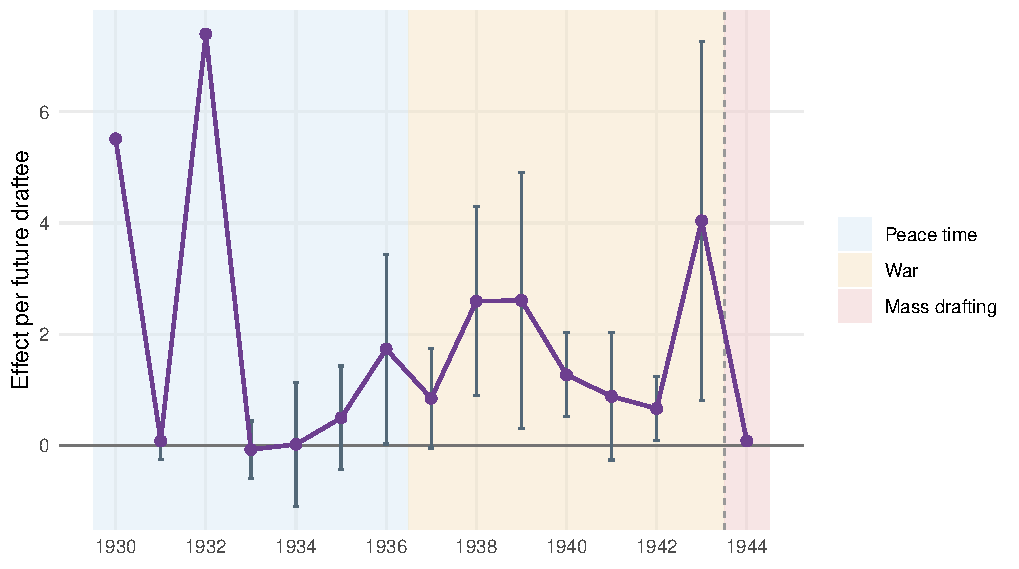
\includegraphics[width=0.84\textwidth]{Results/draft1944_pre_draft_trajectories/draft_intensity_treatment_internal.pdf}
\parbox{0.9\textwidth}{\centering\tiny Separate year-by-year conditional associations with 1944 draft exposure; section and occupation FE and log cumulative male control. Bars show 95\% normal confidence intervals.}
\end{frame}

\begin{frame}[t]{Draft intensity: external hires yearly associations}
\centering
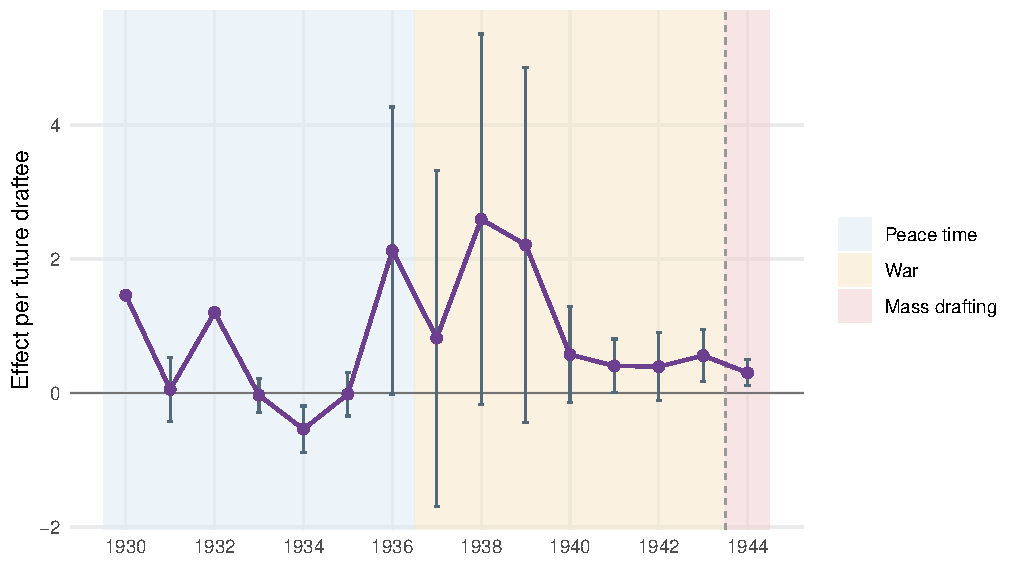
\includegraphics[width=0.84\textwidth]{Results/draft1944_pre_draft_trajectories/draft_intensity_treatment_new_hires.pdf}
\parbox{0.9\textwidth}{\centering\tiny Separate year-by-year conditional associations with 1944 draft exposure; section and occupation FE and log cumulative male control. Bars show 95\% normal confidence intervals.}
\end{frame}

\begin{frame}[t]{Total internal response: yearly associations}
\centering
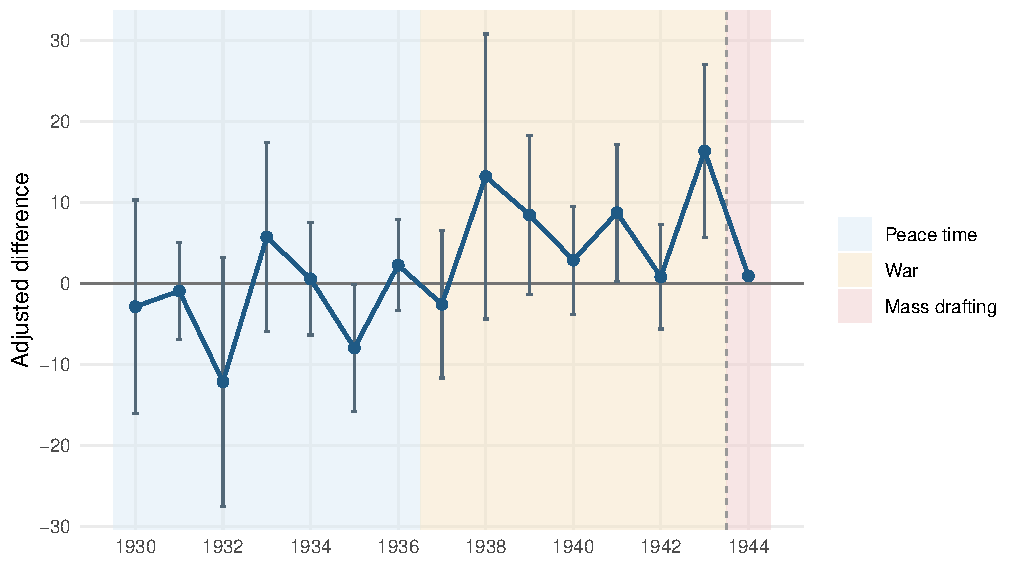
\includegraphics[width=0.84\textwidth]{Results/draft1944_pre_draft_trajectories/within_section_pretrend_internal.pdf}
\parbox{0.9\textwidth}{\centering\tiny Separate year-by-year conditional associations with 1944 draft exposure; section and occupation FE and log cumulative male control. Bars show 95\% normal confidence intervals.}
\end{frame}

\begin{frame}[t]{External hires: yearly associations}
\centering
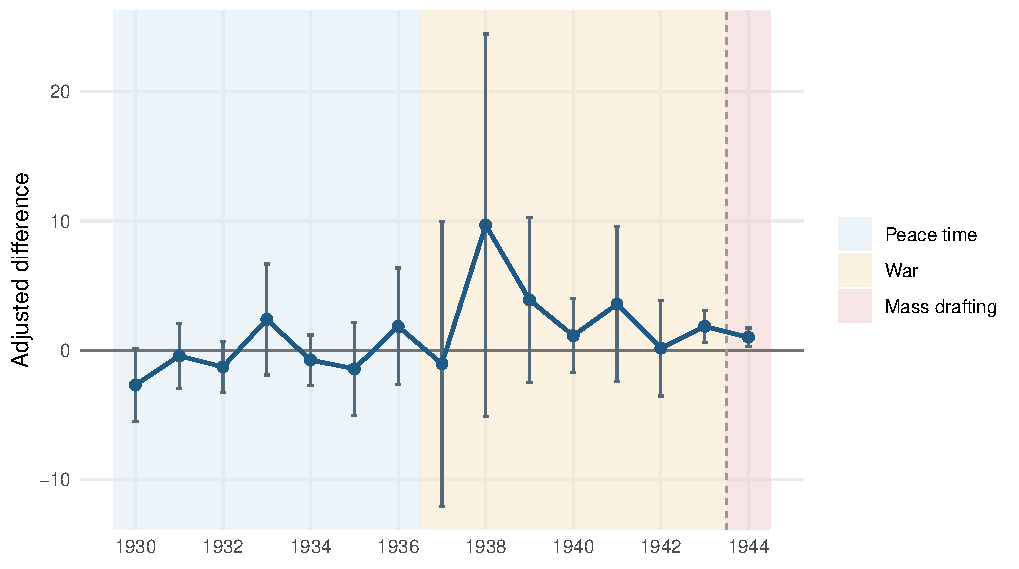
\includegraphics[width=0.84\textwidth]{Results/draft1944_pre_draft_trajectories/within_section_pretrend_new_hires.pdf}
\parbox{0.9\textwidth}{\centering\tiny Separate year-by-year conditional associations with 1944 draft exposure; section and occupation FE and log cumulative male control. Bars show 95\% normal confidence intervals.}
\end{frame}
